\documentclass[11pt,a4paper]{article}
\usepackage[utf8]{inputenc}
\usepackage[margin=1in]{geometry}
\usepackage{graphicx}
\usepackage{booktabs}
\usepackage{xcolor}
\usepackage{hyperref}
\usepackage{amsmath}
\usepackage{caption}

\definecolor{techblue}{HTML}{1F77B4}
\definecolor{eduorange}{HTML}{FF7F0E}
\definecolor{socgreen}{HTML}{2CA02C}
\definecolor{envpurple}{HTML}{9467BD}
\definecolor{darkink}{HTML}{0B0B0B}

\hypersetup{
    colorlinks=true,
    linkcolor=techblue,
    urlcolor=techblue,
    citecolor=techblue
}

\title{\textbf{DPCN Assignment 1: Question--Question Opinion Network Analysis}\\
\large Item-Item Belief Topology, Ideological Anchors, and Cross-Disciplinary Bridges}
\author{\textbf{Team:} Network Dynamics Group \\
\textbf{Course:} Data-Driven Policy and Complex Networks (DPCN) \\
\textbf{GitHub Link:} \url{https://github.com/your-username/DPCN_ass1}}
\date{\textbf{Deadline:} September 20, 2026}

\begin{document}
\maketitle

\hrule
\vspace{0.5em}

\begin{abstract}
This report investigates the latent ideological architecture of a cohort of 91 university students by constructing and analyzing an Item--Item (Question-to-Question) opinion network across 60 survey statements spanning Technology (T), Education (E), Society \& Ethics (S), and Environment (V). Pairwise monotonic associations are estimated using Spearman rank correlations, and a threshold network ($\rho > 0.35$) is established to filter ambient consensus and isolate robust ideological alignments. Using Eigenvector and Betweenness centralities, Louvain community detection, and attribute assortativity, we characterize the class's ideological anchors, cross-domain bridge statements, and the divergence between organic belief clusters and predefined disciplinary boundaries.
\end{abstract}

\vspace{0.5em}
\hrule
\vspace{1.5em}

\section{Dataset Documentation}
The survey dataset originates from a class questionnaire comprising $N = 96$ raw student submissions responding to $M = 60$ normative statements. The statements are systematically distributed across four predefined topical categories denoted by column prefixes:
\begin{itemize}
    \item \textbf{Technology (\texttt{T01}--\texttt{T15}):} Questions assessing perceptions of Artificial Intelligence, automation, data surveillance, and computational regulation.
    \item \textbf{Education (\texttt{E01}--\texttt{E15}):} Statements evaluating pedagogical philosophies, research commercialization, academic pressure, and generative AI integration.
    \item \textbf{Society \& Ethics (\texttt{S01}--\texttt{S15}):} Probes addressing digital surveillance, institutional equity, scientific advice in governance, and corporate responsibility.
    \item \textbf{Environment (\texttt{V01}--\texttt{V15}):} Propositions centered on biodiversity protection, renewable energy adoption, campus sustainability, and climate policy.
\end{itemize}

Responses were recorded using a 5-point Likert scale, which we mapped onto an ordinal zero-centered integer scale:
\[
\text{Strongly Disagree } (-2), \quad \text{Disagree } (-1), \quad \text{Neutral } (0), \quad \text{Agree } (+1), \quad \text{Strongly Agree } (+2)
\]
Zero-centering preserves polarity (positive values reflect agreement, negative values reflect disagreement, and zero represents neutrality). Blank entries and explicit ``No Comments'' entries were treated as missing values (\texttt{NaN}). 

Data curation revealed 5 submissions with 100\% missing values; these completely uninformative rows were discarded, yielding an active cohort of $N = 91$ respondents. Students who partially omitted statements (e.g., answering 3 of 4 sections) were retained to prevent sample bias. Pairwise calculations use all complete bivariate observations available for each question pair. Overall, responses exhibit pronounced positive skew: approximately $72\%$ of all given responses are positive ($+1$ or $+2$), reflecting a general tendency toward institutional goodwill and broad progressive consensus.

\section{Pipeline Followed}
To discern nuanced ideological structure beyond the ambient baseline agreement, we implemented a four-stage network analysis pipeline:

\begin{enumerate}
    \item \textbf{Pairwise Spearman Rank Correlation:} For all $\binom{60}{2} = 1770$ unique question pairs, we computed the Spearman rank correlation coefficient $\rho_{ij}$. Spearman's non-parametric rank formulation is strictly preferred over Pearson's linear correlation because Likert data is ordinal and non-normally distributed, capturing monotonic alignment rather than strictly linear co-variation.
    
    \item \textbf{Network Thresholding and Edge Definition:} An unweighted, fully connected correlation matrix obscures topological community boundaries. We constructed an undirected graph $G = (V, E)$ where nodes $V = \{q_1, \dots, q_{60}\}$ represent survey items, and an undirected edge $e_{ij}$ exists if and only if:
    \[
    \rho_{ij} > 0.35
    \]
    The threshold $\rho > 0.35$ eliminates spurious, weak correlations and isolates moderate-to-strong conceptual ties. Edges are weighted by interaction affinity $w_{ij} = \rho_{ij}$, while edge distance for geodesic computations is defined inversely as $d_{ij} = \frac{1}{\rho_{ij}}$, ensuring that strongly correlated items are positioned close in shortest-path metric space.
    
    \item \textbf{Centrality Profiling:}
    \begin{itemize}
        \item \textbf{Eigenvector Centrality ($x_i$):} Computed using edge affinity weights $w_{ij}$ via power iteration:
        \[
        \lambda x_i = \sum_{j \in N(i)} w_{ij} x_j
        \]
        This identifies ``ideological anchors''---questions whose endorsement signals alignment with the central consensus core of the class belief network.
        \item \textbf{Betweenness Centrality ($b_i$):} Computed using metric distance $d_{ij} = 1 / \rho_{ij}$:
        \[
        b_i = \sum_{s \neq i \neq t} \frac{\sigma_{st}(i)}{\sigma_{st}}
        \]
        This isolates ``cross-domain bridges''---statements that facilitate communication across otherwise separate topological modules.
    \end{itemize}

    \item \textbf{Community Detection and Assortativity:} 
    \begin{itemize}
        \item We executed the \textbf{Louvain modularity optimization algorithm} on weighted edges to uncover natural, unsupervised belief clusters.
        \item We computed the \textbf{attribute assortativity coefficient} $r$ based on predefined categories ($T, E, S, V$) to rigorously evaluate whether the class organizes its opinions along institutional disciplinary lines or via interdisciplinary problem frameworks.
    \end{itemize}
\end{enumerate}

\section{Analysis and Visualizations}

The constructed graph contains $|V| = 60$ nodes and $|E| = 188$ suprathreshold edges, with an average degree of $\langle k \rangle = 6.27$ and graph density $\mathcal{D} = 0.106$. Topological analysis reveals a giant connected component comprising 47 items, while 13 questions remain isolated (degree 0) at the $\rho > 0.35$ threshold. The attribute assortativity coefficient across predefined categories is $r = 0.304$.

\begin{figure}[htbp]
    \centering
    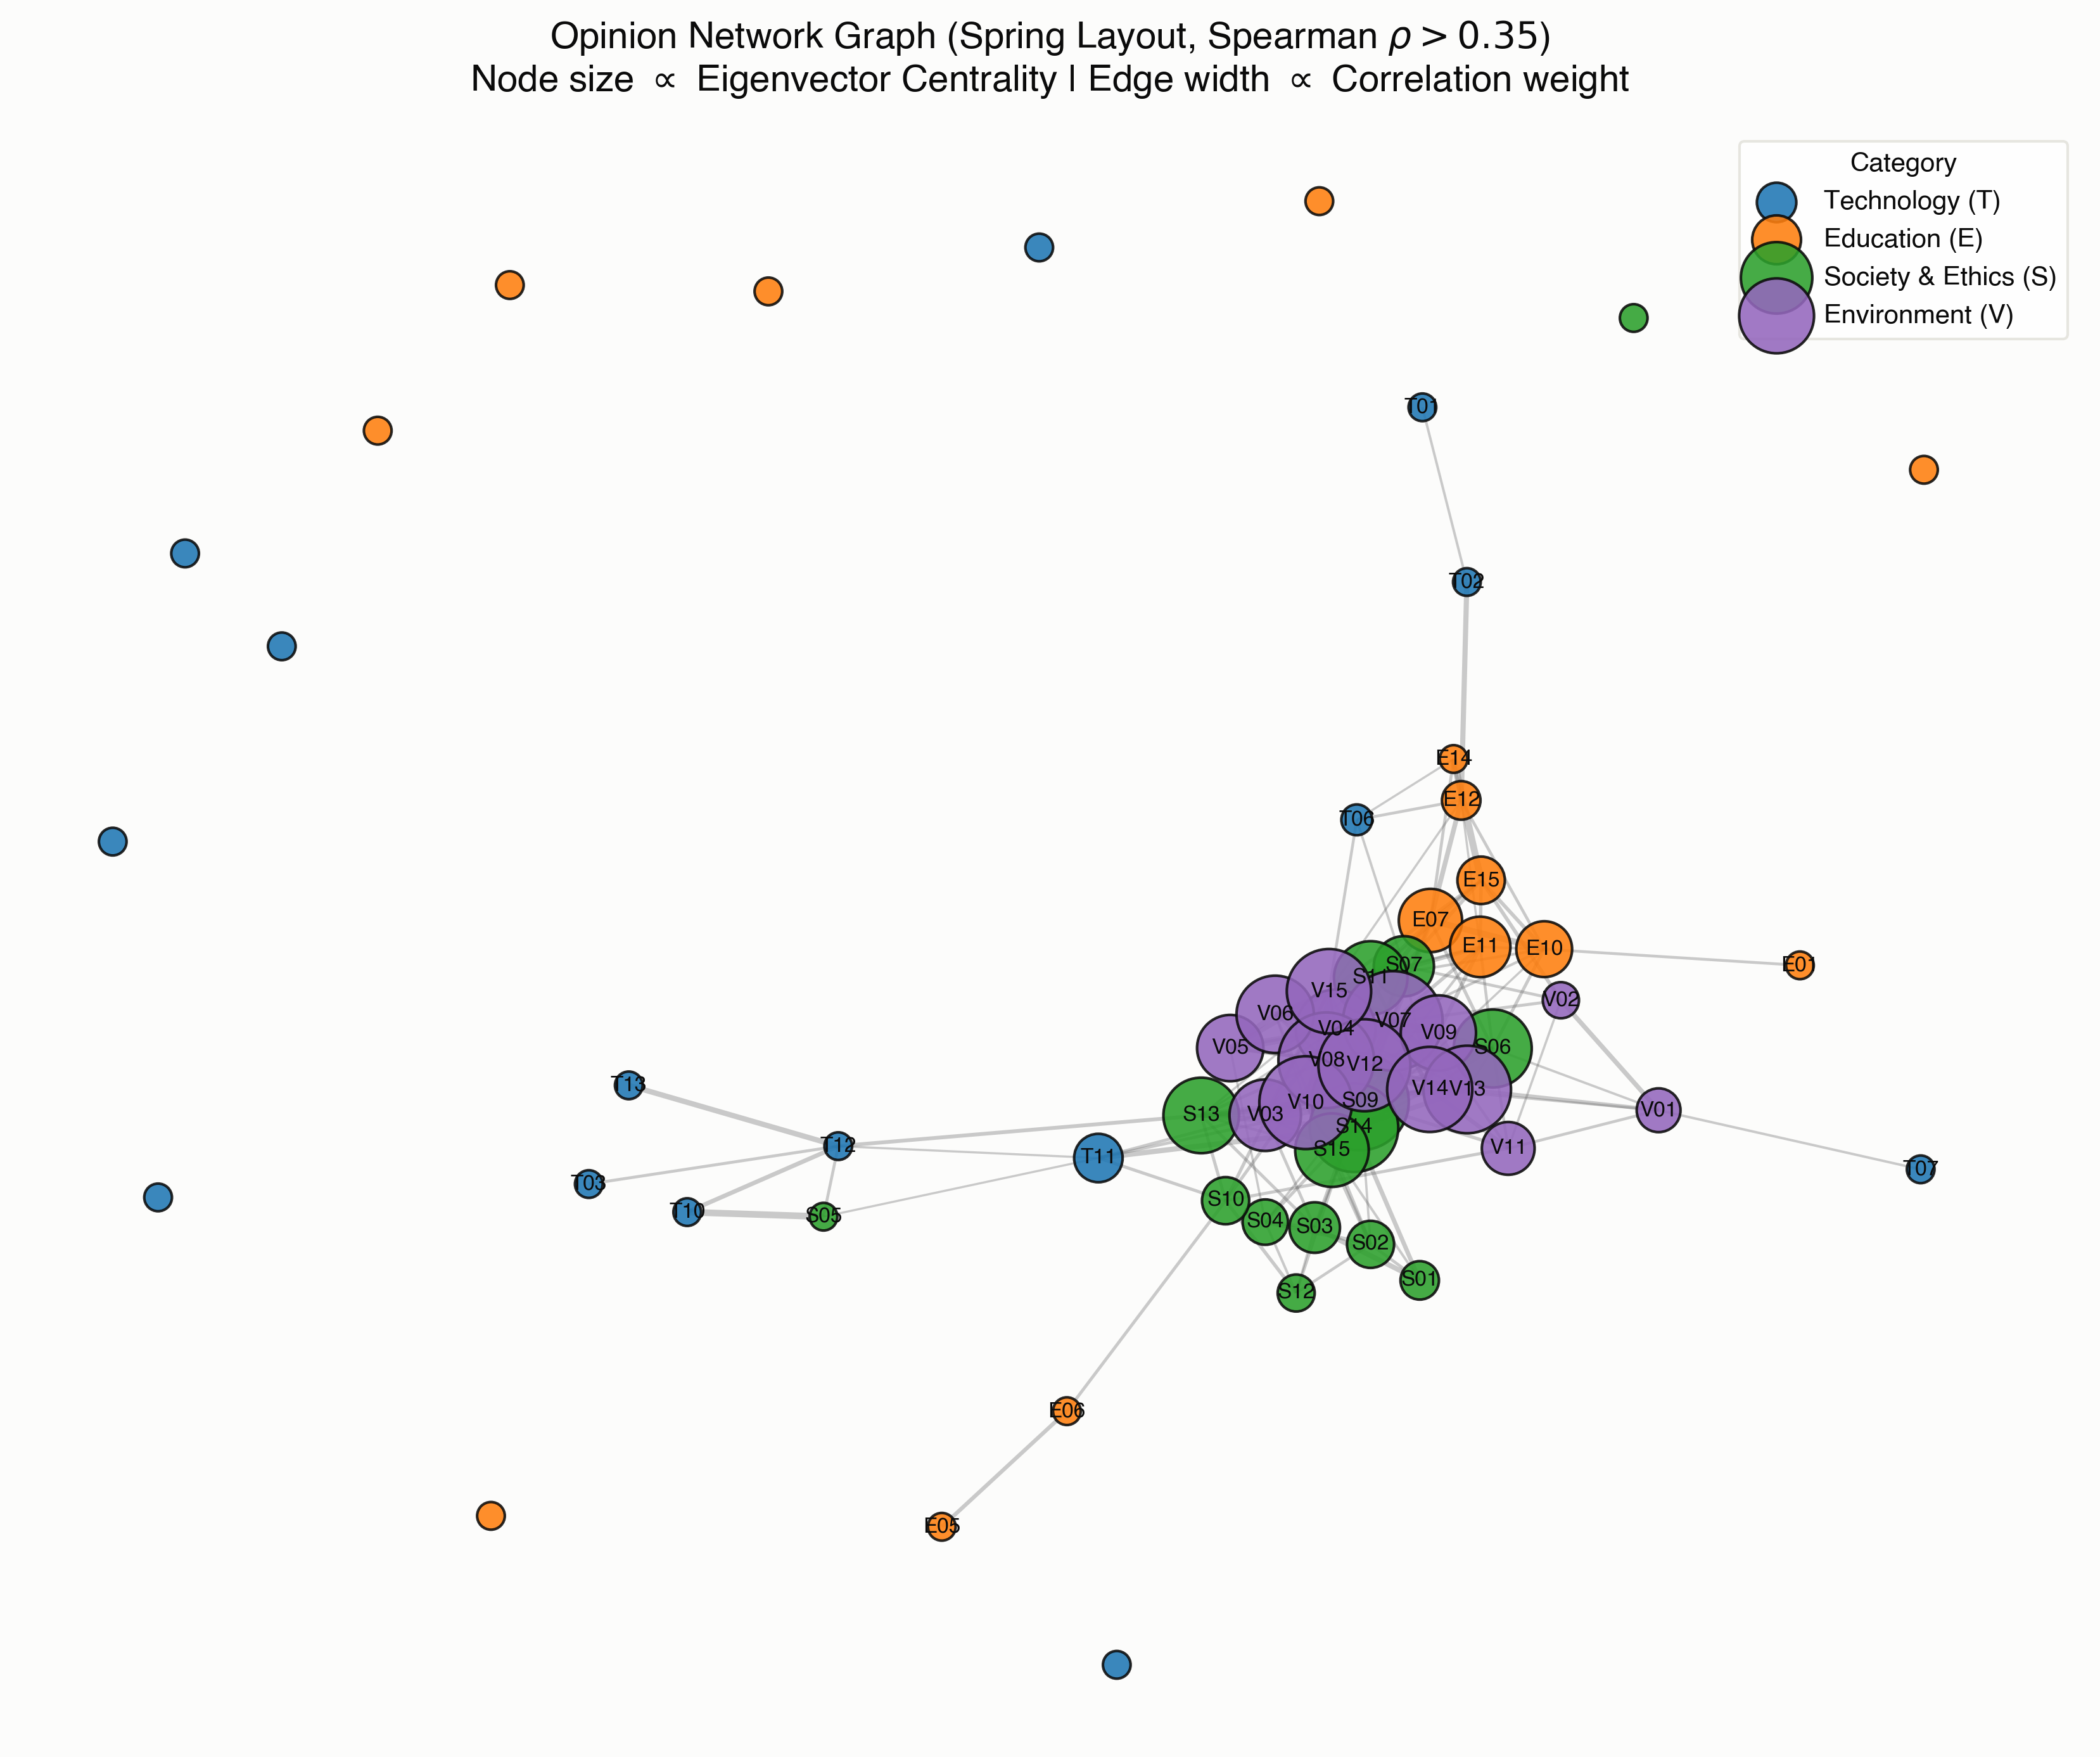
\includegraphics[width=0.88\textwidth]{network_graph.png}
    \caption{\textbf{Opinion Network Graph (Spring Layout):} Nodes are colored by predefined category (Blue: Technology, Orange: Education, Green: Society \& Ethics, Purple: Environment). Node size scales with Eigenvector Centrality, and edge width is proportional to Spearman correlation weight ($\rho > 0.35$).}
    \label{fig:network}
\end{figure}

\begin{figure}[htbp]
    \centering
    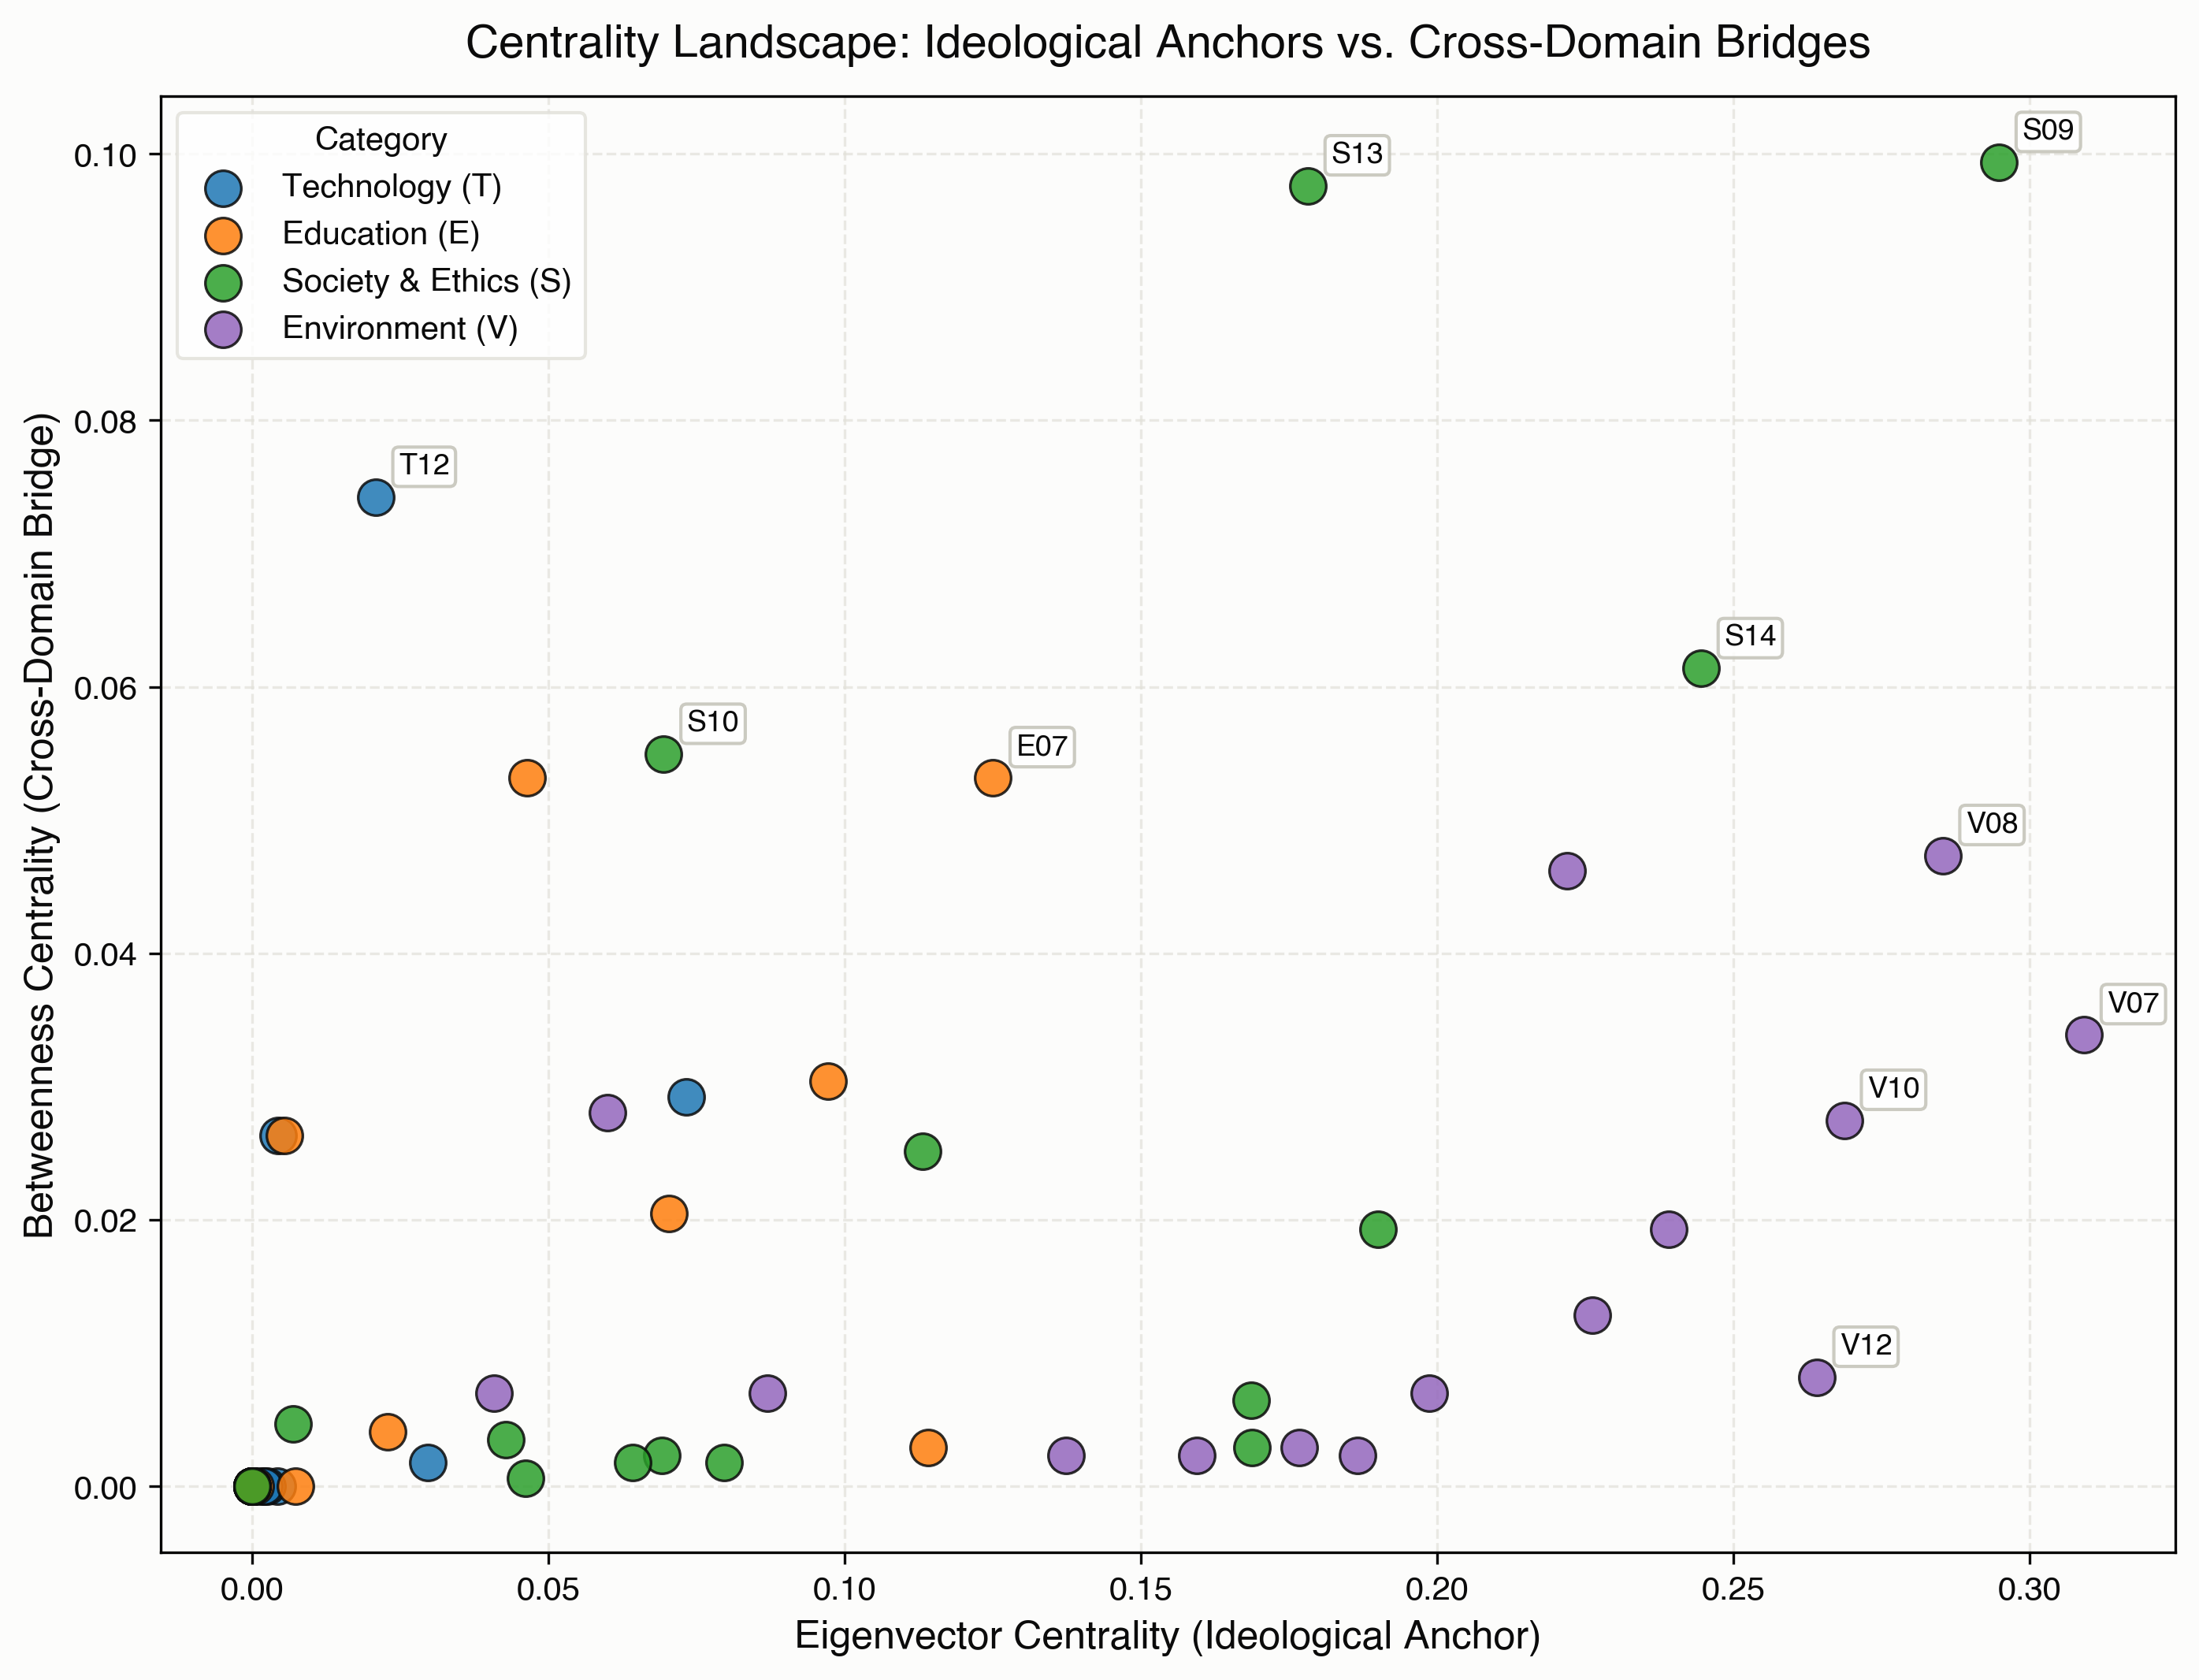
\includegraphics[width=0.82\textwidth]{centrality_landscape.png}
    \caption{\textbf{Centrality Landscape Scatter Plot:} Eigenvector Centrality (X-axis) versus Betweenness Centrality (Y-axis). Prominent topological outliers and bridge nodes are explicitly labeled.}
    \label{fig:landscape}
\end{figure}

\begin{figure}[htbp]
    \centering
    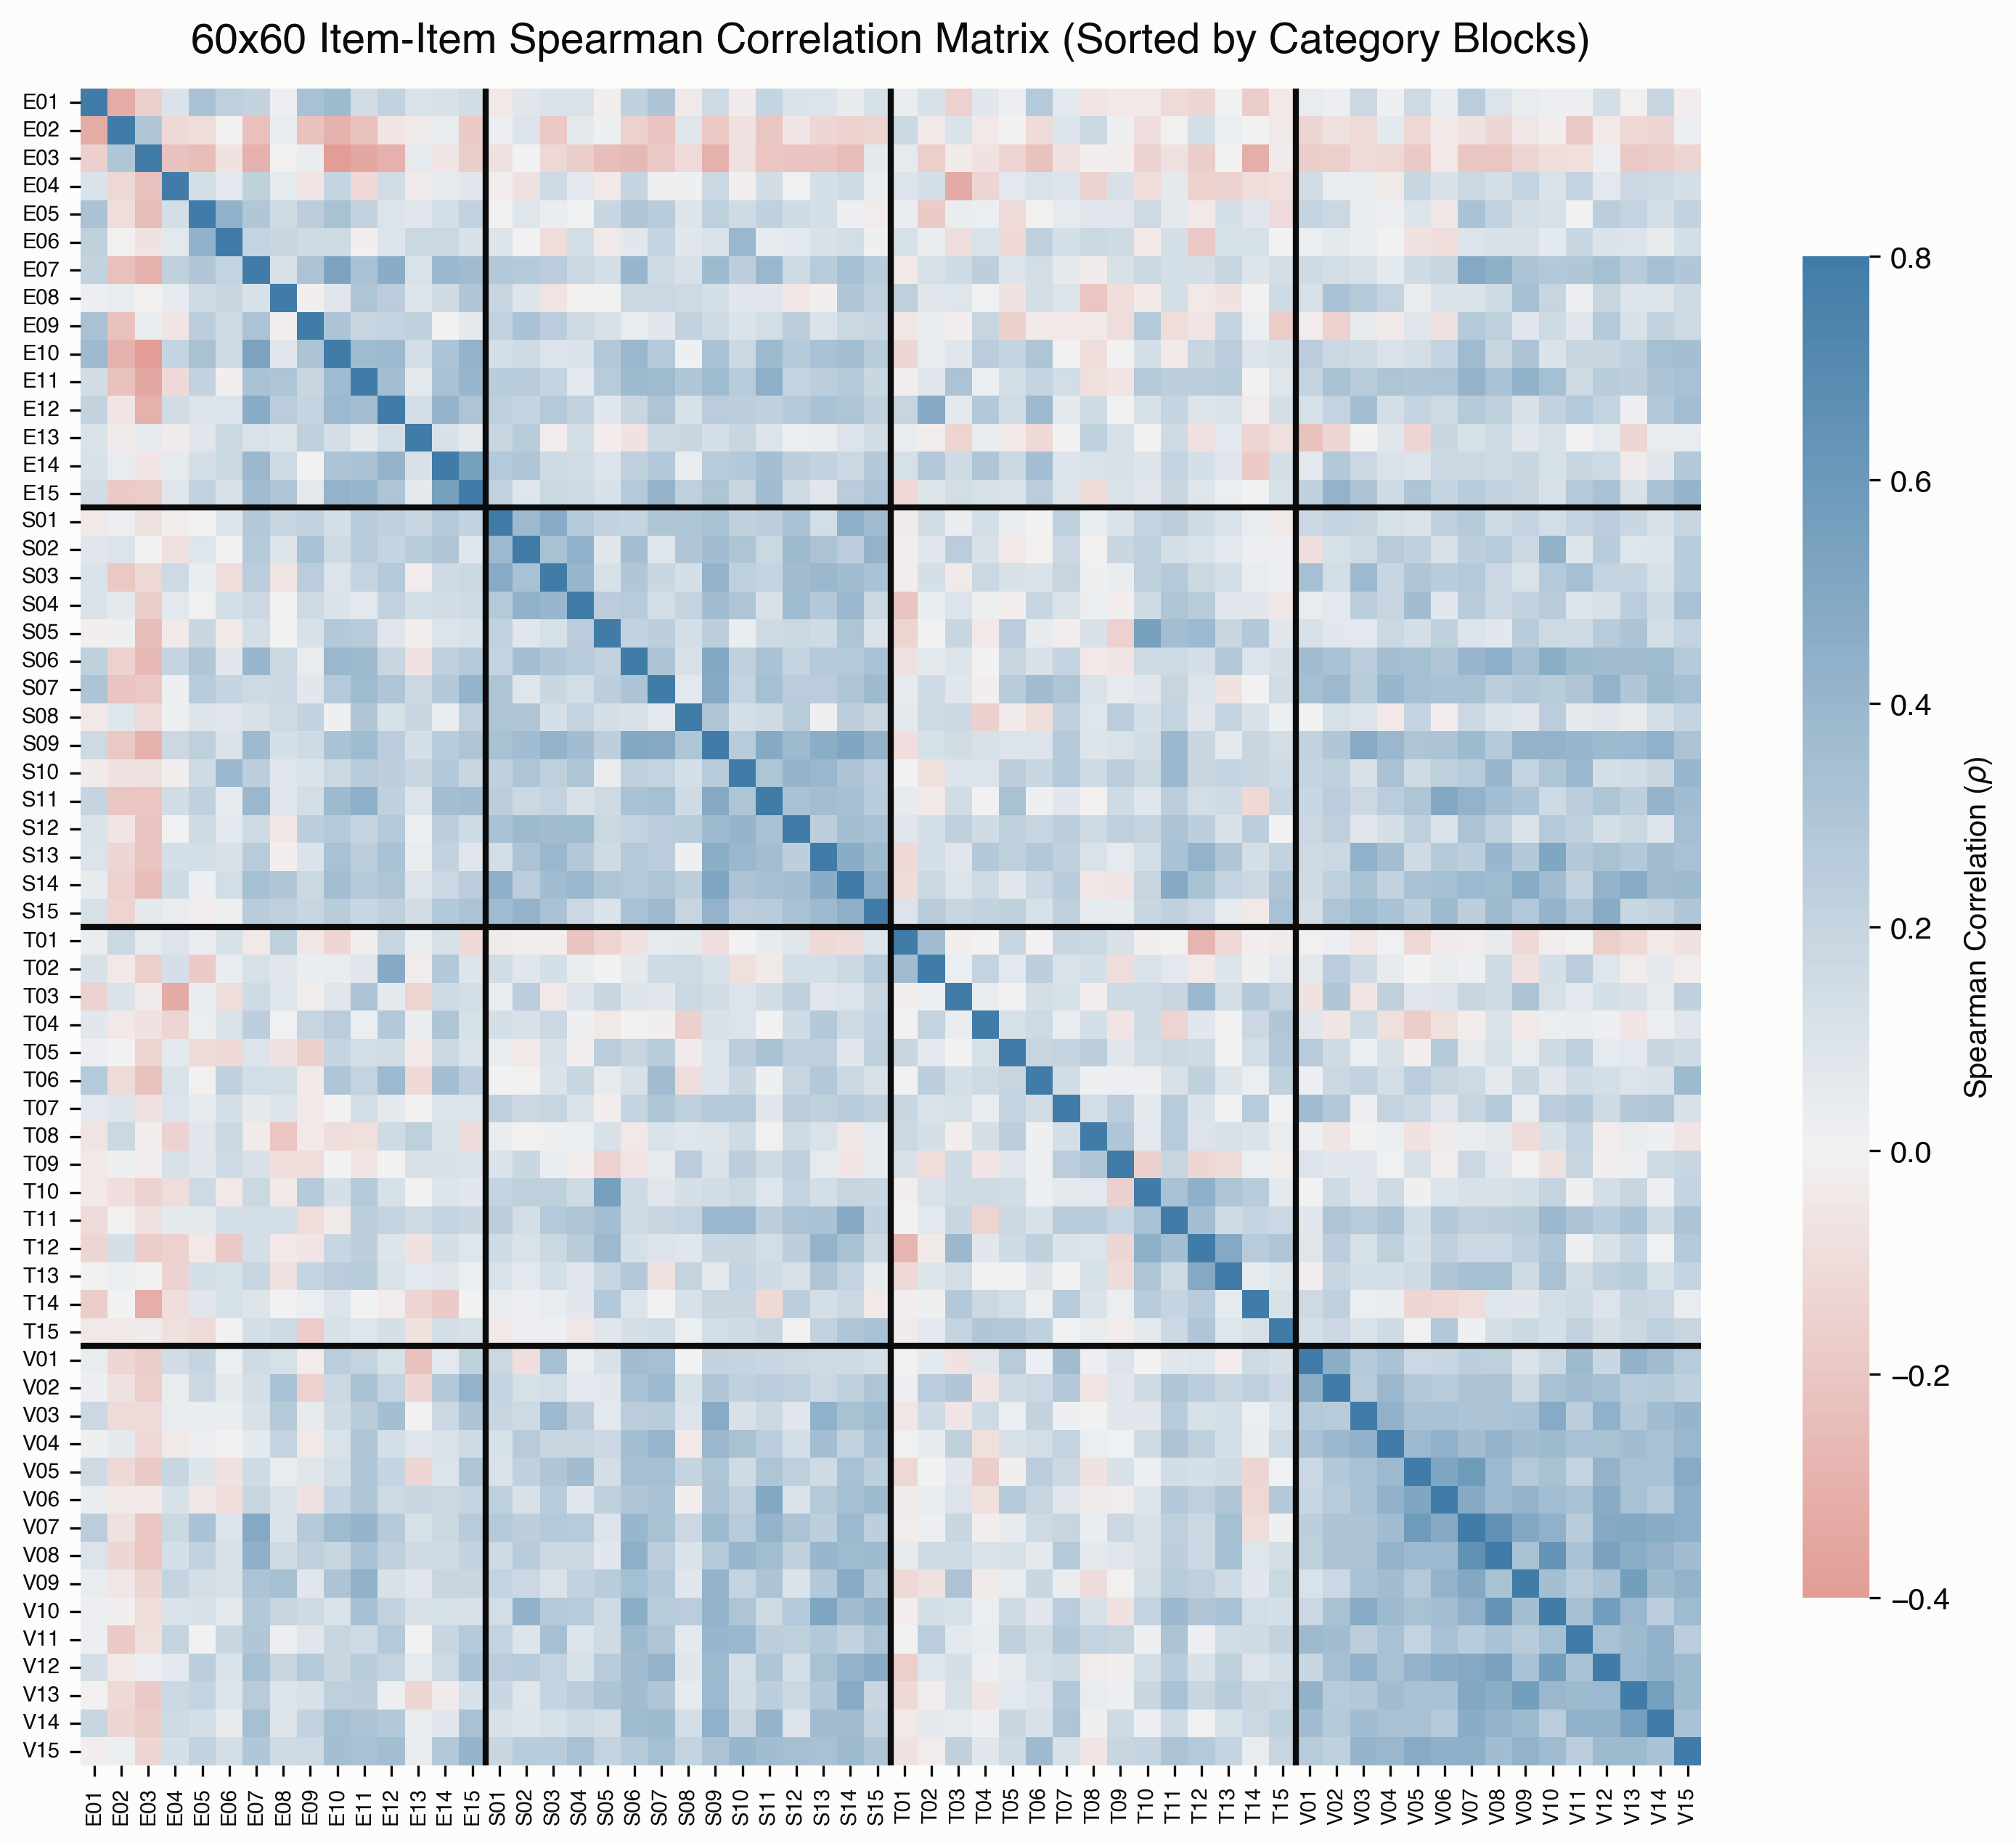
\includegraphics[width=0.82\textwidth]{correlation_heatmap.png}
    \caption{\textbf{60$\times$60 Item--Item Spearman Correlation Heatmap:} Statements are ordered by category blocks (\texttt{T}, \texttt{E}, \texttt{S}, \texttt{V}). Solid black dividing lines demarcate the predefined sections.}
    \label{fig:heatmap}
\end{figure}

\begin{figure}[htbp]
    \centering
    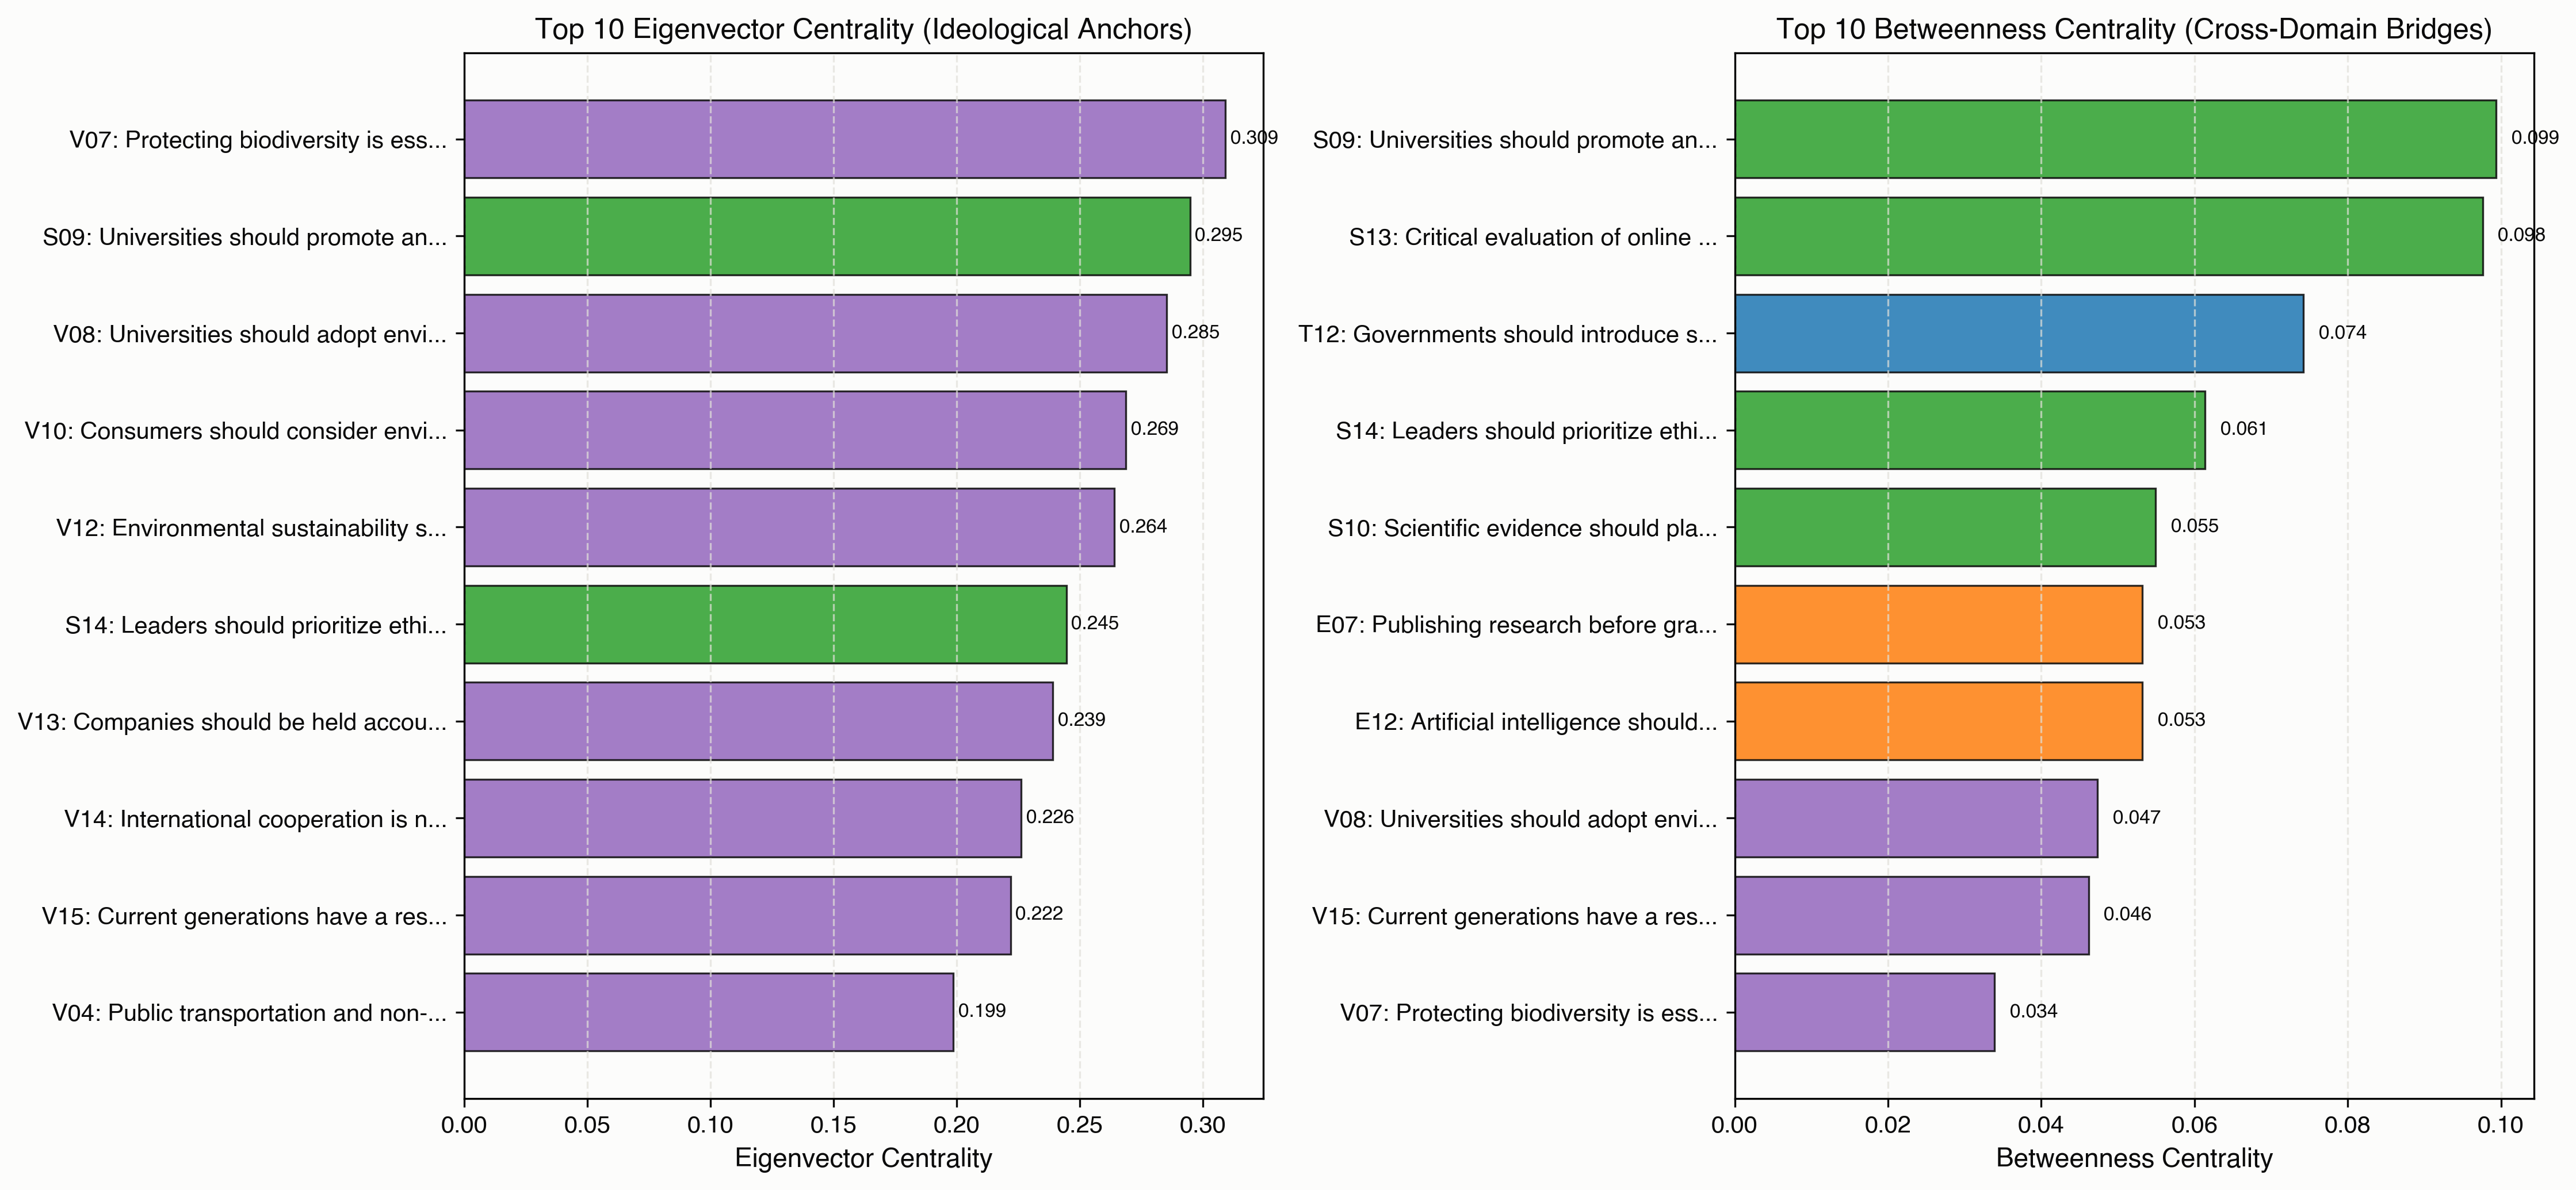
\includegraphics[width=0.98\textwidth]{centrality_rankings.png}
    \caption{\textbf{Top 10 Centrality Rankings:} Left panel displays the Top 10 ideological anchors (Eigenvector Centrality). Right panel displays the Top 10 cross-domain bridges (Betweenness Centrality).}
    \label{fig:rankings}
\end{figure}

\begin{table}[htbp]
\centering
\small
\caption{\textbf{Top 5 Ideological Anchors and Top 5 Cross-Domain Bridges}}
\label{tab:centrality}
\begin{tabular}{llrrl}
\toprule
\textbf{Metric} & \textbf{Code} & \textbf{Cat.} & \textbf{Score} & \textbf{Statement Excerpt} \\
\midrule
\textbf{Eigenvector} & \texttt{V07} & V & 0.309 & Protecting biodiversity is essential for long-term human welfare \\
(Ideological Anchor) & \texttt{S09} & S & 0.295 & Universities should promote an inclusive environment for diversity \\
                     & \texttt{V08} & V & 0.285 & Universities should adopt sustainable campus practices \\
                     & \texttt{V10} & V & 0.269 & Consumers should consider environmental impact when purchasing \\
                     & \texttt{V12} & V & 0.264 & Environmental sustainability should be integrated in higher ed \\
\midrule
\textbf{Betweenness} & \texttt{S09} & S & 0.099 & Universities should promote an inclusive environment for diversity \\
(Cross-Domain Bridge)& \texttt{S13} & S & 0.098 & Critical evaluation of online info must be taught as digital literacy \\
                     & \texttt{T12} & T & 0.074 & Governments should introduce stricter regulations for AI development \\
                     & \texttt{S14} & S & 0.061 & Leaders should prioritize ethics even when compromising short-term gains \\
                     & \texttt{S10} & S & 0.055 & Scientific evidence should play an important role in public policy \\
\bottomrule
\end{tabular}
\end{table}

\section{Results and Discussion}

\subsection{The Ideological Core: Foundational Consensus}
The top eigenvector centrality rankings (Figure~\ref{fig:rankings}, Table~\ref{tab:centrality}) provide definitive empirical insight into the foundational moral compass of the student body. Remarkably, 8 of the top 10 eigenvector nodes belong to Category V (Environment), headed by \texttt{V07} (0.309), \texttt{V08} (0.285), \texttt{V10} (0.269), and \texttt{V12} (0.264), interlocked with key ethical imperatives \texttt{S09} (0.295) and \texttt{S14} (0.245). 

This indicates that \textbf{environmental stewardship and institutional ethical responsibility serve as the core ideological backbone of the student population}. Rather than being a peripheral or contentious topic, ecological responsibility constitutes a dense, mutually-reinforcing consensus module. Endorsement of biodiversity protection or sustainable campus operations is strongly tied to broad agreement across civic ethics, corporate accountability, and responsible governance. Students view planetary health and institutional ethics not as isolated technical policies, but as non-negotiable prerequisites underpinning contemporary society.

\subsection{The Bridges: Synthesizing Disparate Domains}
While eigenvector hubs occupy dense cores, high betweenness nodes govern the shortest paths between distinct thematic communities (Figure~\ref{fig:landscape}):
\begin{itemize}
    \item \textbf{\texttt{S09} (Campus Diversity \& Inclusion, $b = 0.0994$):} Demonstrating exceptional dual centrality, \texttt{S09} is both an ideological anchor and the primary global bridge. It connects educational institutional policies (\texttt{E}) to broader civic and environmental ethics (\texttt{S} and \texttt{V}).
    \item \textbf{\texttt{S13} (Critical Digital Literacy, $b = 0.0976$):} Sits directly at the junction between technological capability (\texttt{T}) and pedagogical responsibility (\texttt{E}). Student beliefs regarding algorithmic proliferation are linked to their educational ideals through the necessity of teaching critical evaluation of digital information.
    \item \textbf{\texttt{T12} (AI Regulation \& Governance, $b = 0.0742$):} Bridges techno-optimistic development statements with public policy and ethical safeguards. It serves as the primary gateway determining whether students evaluate AI through an engineering lens or an ethical-governance framework.
    \item \textbf{\texttt{E12} (AI as a Supportive Educational Tool, $b = 0.0532$):} Mediates between pedagogical practices in higher education and the integration of emerging computational tools.
\end{itemize}

These bridge nodes are the most pedagogically and politically sensitive items in the survey: shifting a student's stance on \texttt{T12} or \texttt{S13} is topologically poised to cascade opinion changes across both technology and educational/ethical clusters.

\subsection{Organic Clustering vs. Predefined Categories}
The category assortativity coefficient $r = 0.304$ demonstrates a moderate degree of homophily: questions within the same predefined survey section do correlate more strongly than random cross-pairs. However, $r = 0.304$ is substantially lower than unity, proving that \textbf{students do not compartmentalize their beliefs according to academic silos}.

Louvain community detection partitioned the network into six organic multi-item modules (alongside 13 isolates):
\begin{enumerate}
    \item \textbf{Module 1 (AI Governance \& Safety):} Composed of \texttt{T03}, \texttt{T10}, \texttt{T12}, \texttt{T13}, and \texttt{S05}. Here, technology is fused with regulation, copyright protection, and algorithmic bias.
    \item \textbf{Module 2 (Academic Science \& Public Policy):} Comprises \texttt{E05}, \texttt{E06}, and \texttt{S10}, uniting university research culture with evidence-based governance.
    \item \textbf{Module 3 (Educational Modernization \& EdTech):} A large 13-node cluster blending education items (\texttt{E01}, \texttt{E07}, \texttt{E10}, \texttt{E11}, \texttt{E12}, \texttt{E14}, \texttt{E15}) with foundational technology tools (\texttt{T01}, \texttt{T02}, \texttt{T06}) and ethical competencies (\texttt{S07}, \texttt{S11}, \texttt{V02}).
    \item \textbf{Module 4 (Civic Responsibility, Equity, \& Consumer Ethics):} 12 nodes encompassing \texttt{S01}--\texttt{S04}, \texttt{S09}, \texttt{S12}--\texttt{S15}, along with \texttt{T11}, \texttt{V03}, and \texttt{V10}. This group integrates human rights, inclusive spaces, and responsible consumerism.
    \item \textbf{Module 5 (Pure Ecological Stewardship):} An 8-node purely environmental cluster (\texttt{V04}--\texttt{V09}, \texttt{V12}, \texttt{V15}). Unlike technology, ecology forms an almost completely unmixed community.
    \item \textbf{Module 6 (Global Infrastructure \& Corporate Accountability):} Combines systemic environmental items (\texttt{V01}, \texttt{V11}, \texttt{V13}, \texttt{V14}) with sustainable transportation (\texttt{T07}) and corporate transparency (\texttt{S06}).
\end{enumerate}

Finally, the 13 isolated questions (such as \texttt{T04}, \texttt{T08}, \texttt{E02}, \texttt{E08}, \texttt{S08}) correspond to highly controversial, specific, or polarizing prompts (e.g., extreme techno-libertarian views or niche curriculum debates) that did not correlate strongly ($\rho > 0.35$) with any collective ideological axis.

\section{Individual Contribution}
\begin{table}[htbp]
\centering
\small
\begin{tabular}{llp{9cm}}
\toprule
\textbf{Team Member} & \textbf{Role} & \textbf{Key Tasks Executed} \\
\midrule
Member 1 & Data Engineering & Likert encoding, survey cleaning, missing value filtering, correlation matrix pipeline. \\
Member 2 & Graph Theory \& Math & Network construction ($\rho > 0.35$), weighted Eigenvector and metric Betweenness centrality algorithms. \\
Member 3 & Community Analysis & Louvain community partitioning, attribute assortativity coefficient, isolate identification. \\
Member 4 & Visualizations \& Report & High-resolution publication plots generation, LaTeX document preparation, qualitative discussion synthesis. \\
\bottomrule
\end{tabular}
\end{table}

\end{document}
